% mnras_template.tex 
%
% LaTeX template for creating an MNRAS paper
%
% v3.0 released 14 May 2015
% (version numbers match those of mnras.cls)
%
% Copyright (C) Royal Astronomical Society 2015
% Authors:
% Keith T. Smith (Royal Astronomical Society)

% Change log
%
% v3.0 May 2015
%    Renamed to match the new package name
%    Version number matches mnras.cls
%    A few minor tweaks to wording
% v1.0 September 2013
%    Beta testing only - never publicly released
%    First version: a simple (ish) template for creating an MNRAS paper

%%%%%%%%%%%%%%%%%%%%%%%%%%%%%%%%%%%%%%%%%%%%%%%%%%
% Basic setup. Most papers should leave these options alone.
\documentclass[fleqn,usenatbib]{mnras}

% MNRAS is set in Times font. If you don't have this installed (most LaTeX
% installations will be fine) or prefer the old Computer Modern fonts, comment
% out the following line
\usepackage{newtxtext,newtxmath}
% Depending on your LaTeX fonts installation, you might get better results with one of these:
%\usepackage{mathptmx}
%\usepackage{txfonts}

% Use vector fonts, so it zooms properly in on-screen viewing software
% Don't change these lines unless you know what you are doing
\usepackage[T1]{fontenc}

% Allow "Thomas van Noord" and "Simon de Laguarde" and alike to be sorted by "N" and "L" etc. in the bibliography.
% Write the name in the bibliography as "\VAN{Noord}{Van}{van} Noord, Thomas"
\DeclareRobustCommand{\VAN}[3]{#2}
\let\VANthebibliography\thebibliography
\def\thebibliography{\DeclareRobustCommand{\VAN}[3]{##3}\VANthebibliography}


%%%%% AUTHORS - PLACE YOUR OWN PACKAGES HERE %%%%%
\usepackage{indentfirst}
\usepackage{physics}
\usepackage{lineno}
\linenumbers
\usepackage{ulem}
% Only include extra packages if you really need them. Common packages are:
\usepackage{graphicx}	% Including figure files
\usepackage{amsmath}	% Advanced maths commands
\usepackage{amssymb}	% Extra maths symbols
\usepackage{xcolor}
%%%%%%%%%%%%%%%%%%%%%%%%%%%%%%%%%%%%%%%%%%%%%%%%%%

%%%%% AUTHORS - PLACE YOUR OWN COMMANDS HERE %%%%%

% Please keep new commands to a minimum, and use \newcommand not \def to avoid
% overwriting existing commands. Example:
%\newcommand{\pcm}{\,cm$^{-2}$}	% per cm-squared

%%%%%%%%%%%%%%%%%%%%%%%%%%%%%%%%%%%%%%%%%%%%%%%%%%

%%%%%%%%%%%%%%%%%%% TITLE PAGE %%%%%%%%%%%%%%%%%%%

% Title of the paper, and the short title which is used in the headers.
% Keep the title short and informative.
\normalem
\title[Metacalibration for the Roman High-Latitude Imaging Survey]{Weak gravitational lensing shear estimates with \textsc{metacalibration} for the \emph{Roman} High-Latitude Imaging Survey}

% The list of authors, and the short list which is used in the headers.
% If you need two or more lines of authors, add an extra line using \newauthor
\author[M. Yamamoto et al.]{
Masaya Yamamoto,$^{1}$\thanks{E-mail: masaya.yamamoto@duke.edu}
Michael A. Troxel,$^{1}$
Mike Jarvis,$^{2}$
Rachel Mandelbaum,$^{3}$
Christopher Hirata,$^{4,5,6}$
 et al.\\
% List of institutions
$^{1}$Department of Physics, Duke University, Durham, NC, 27710\\
$^{2}$Department of Physics and Astronomy, University of Pennsylvania, Philadelphia, PA 19104, USA\\
$^{3}$McWilliams Center for Cosmology, Department of Physics, Carnegie Mellon University, Pittsburgh, Pennsylvania 15213, USA\\
$^{4}$Center for Cosmology and Astro-Particle Physics, The Ohio State University, 191 West Woodruff Avenue, Columbus, OH 43210, USA\\
$^{5}$Department of Physics, The Ohio State University, 191 West Woodruff Avenue, Columbus, OH 43210, USA\\
$^{6}$Department of Astronomy, The Ohio State University, 140 West 18th Avenue, Columbus, OH 43210, USA\\
}

% These dates will be filled out by the publisher
\date{Accepted XXX. Received YYY; in original form ZZZ}

% Enter the current year, for the copyright statements etc.
\pubyear{2015}

% Don't change these lines
\begin{document}
\label{firstpage}
\pagerange{\pageref{firstpage}--\pageref{lastpage}}
\maketitle

% Abstract of the paper
\begin{abstract}
We investigate the performance of the \textsc{metacalibration} shear calibration framework using image simulations for the \emph{Nancy Grace Roman} Space Telescope (\emph{Roman}) reference High-Latitude Imaging Survey (HLIS). These large-scale realistic image simulations are necessary to measure shear bias to confirm that the requirements of the instrument and the overall weak lensing survey strategy are met. The weak lensing program of the \emph{Roman} mission requires the galaxy shapes to be calibrated within about 0.03\%. To reach this goal, we can test our calibration process with these simulations and ultimately isolate the sources where these residual shear biases arise. In this work, we incorporate several new realistic processing-pipeline updates necessary to calibrate shear with a better precision relative to the previous version of the simulations and show first results for the reference HLIS using \textsc{metacalibration}. We find that \textsc{metacalibration} as used in current experiments can significantly reduce the shear calibration bias to the percent level. With the single-epoch images, across all three filters we are able to achieve a multiplicative bias $m=(-1.34\pm 0.67)$\%, while for coadd cutouts, $m=(-2.33\pm 0.64)$\%. In both single-epoch and coadd cases, we find that shape calibration becomes worse with decreasing image sampling factor. Overall, within the current simulation volume, there is evidence that \textsc{metacalibration} as currently implemented will not calibrate shapes with zero shear bias in the \emph{Roman} HLIS and further work on the shear calibration methodology is necessary. In the future, we will need to substantially increase the simulation volume by 400 (about the same size as the survey area of 2000 deg$^{2}$) to reach the precision necessary for the HLIS.
\end{abstract}

% Select between one and six entries from the list of approved keywords.
% Don't make up new ones.
\begin{keywords}
gravitational lensing: weak -- cosmology: observations -- techniques: image processing
\end{keywords}

%%%%%%%%%%%%%%%%%%%%%%%%%%%%%%%%%%%%%%%%%%%%%%%%%%

%%%%%%%%%%%%%%%%% BODY OF PAPER %%%%%%%%%%%%%%%%%%

\section{Introduction}

Since the formulation of a physical cosmological model, more observational evidence has shown that the contents of the universe are mostly in the dark sector (\citealt{2020A&A...633A..69H, 2018PhRvD..98d3528T, 2019PhRvL.122q1301A, 2019PASJ...71...43H, 2021A&A...645A.104A}). Within this sector, dark energy accounts for the accelerating expansion of the universe (e.g., \citealt{1998AJ....116.1009R, 1999AIPC..478..129P}) and the combination of dark energy and dark matter are responsible for the observed growth of large-scale structure (\citealt{2015RPPh...78h6901K, 2017grle.book.....D}). The growth can be studied by carefully reconstructing the paths of the light leaving distant galaxies and going through the regions where mass concentrates in the universe; this physical phenomenon is called gravitational lensing. “Weak” gravitational lensing causes a slight distortion to intrinsic galaxy shapes when observed from the Earth. By detecting millions of these gravitationally lensed galaxies and computing their ensemble distortion levels, we can explore the dark matter density and the amplitude of matter fluctuation in the universe (e.g., \citealt{2001PhR...340..291B}). Measuring these quantities eventually helps us learn about the history of the development of the large-scale structure in the universe. For that reason, weak lensing is one of the most powerful probes in current and near-future imaging surveys to constrain cosmological parameters with high precision. \par


Due to the subtlety in the lensing effect and its systematics-dominant nature in the weak regime, observational efforts have been challenging. Over the past decade, large international collaborations such as the Dark Energy Survey\footnote{\url{http://www.darkenergysurvey.org/}} (DES: \citealt{2005astro.ph.10346T}), the Hyper Supreme-Cam\footnote{\url{http://hsc.mtk.nao.ac.jp/ssp/}} (HSC: \citealt{2018PASJ...70S...4A}), and the Kilo-Degree Survey\footnote{\url{http://kids.strw.leidenuniv.nl/}} (KiDS: \citealt{2013ExA....35...25D}) have been successful at constraining the cosmological parameters, and the precision in calibrating the shapes of distant galaxies has reached a few percent (\citealt{2020arXiv201103408G, 2020arXiv201208567M, 2021A&A...645A.105G}). As we observe more area of the sky and develop better tools (observatories and algorithms), we detect more galaxies, and have already reached the point where statistical and systematic uncertainties are comparable. Thus, near-future Stage IV surveys (\citealt{2006astro.ph..9591A}) such as Euclid\footnote{\url{ http://sci.esa.int/euclid}} (\citealt{2011arXiv1110.3193L}), the Vera C. Rubin Observatory Legacy Survey of Space and Time\footnote{\url{ http://www.lsst.org}} (\emph{Rubin}: \citealt{2009arXiv0912.0201L, 2019ApJ...873..111I}), and the \emph{Nancy Grace Roman} Space Telescope\footnote{\url{https://roman.gsfc.nasa.gov}} (\emph{Roman}: \citealt{2015arXiv150303757S}) require even better control of systematics. In order to understand the systematic uncertainties we face, we must develop realistic image simulations, apply pre-existing shape measurement to the simulated images, and determine any potential residual systematic effects and build a strategy for modifying the calibration methodology to mitigate them.  


Based on our current knowledge, systematic biases for weak lensing science, both observational and astrophysical, can occur at all stages of the imaging survey (e.g., \citealt{2018ARA&A..56..393M}). Particularly, observational systematics can be due to: 
\begin{itemize}
    \item inhomogeneous observing strategy,
    \item instrumentation effects,
    \item post-processing pipelines such as image coaddition and object detection.
\end{itemize} 

Conventionally, these observational systematic biases are realized through a number of simulations and validations, and these propagate into the final galaxy shapes we measure. We quantify this impact as shear calibration bias. There have been several shear calibration and bias mitigation efforts that were proposed by STEP (\citealt{2006MNRAS.368.1323H, 2007MNRAS.376...13M}) and GREAT (\citealt{2010MNRAS.405.2044B, 2013ApJS..205...12K, 2015MNRAS.450.2963M}) challenges, to meet the requirements for the current imaging surveys. In particular, one of the state-of-the-art self-calibration methods, \textsc{metacalibration} (\citealt{2017arXiv170202600H, 2017ApJ...841...24S}) has been shown to be able to substantially reduce the significance of shear bias. It has been confirmed that shear can be calibrated with \textsc{metacalibration} at the few-percent level in DES (\citealt{2018MNRAS.481.1149Z, 2020arXiv201103408G}), without accounting for galaxy blending and detection. Tackling the issue of blending/detection is one key step forward for the DES Y6 analysis and preparatory Rubin LSST work with the shear-dependent detection and calibration technique (\textsc{metadetection}; \citealt{2020ApJ...902..138S}). While the major advantage of \textsc{metacalibration} is that it can be directly applied to real galaxy images without needing to rely on an ensemble calibration from image simulations, limitations for future surveys are not well-known. 

One possible limitation might lie in the effect of undersampled images in space-based surveys like \emph{Euclid} and \emph{Roman}, which will operate at its diffraction-limit (\citealt{2013PASP..125.1496S}). The PSF needs to be interpolated and estimated from well-sampled images to deconvolve and measure shapes, because the \emph{Roman} PSF has a complex structure that cannot be captured in the original undersampled images. It is, therefore, necessary to build a robust strategy to reconstruct well-sampled images to estimate the PSF to allow unbiased shape measurement.
Recently, \cite{2021MNRAS.502.4048K} (hereafter K21) addressed this potential issue of the limitations of \textsc{metacalibration} on undersampled images in \emph{Euclid} image simulations. They found that for the \emph{Euclid} mission the shear estimate with \textsc{metacalibration} is biased by about 1$\%$. It is mentioned that their result could be extended to the \emph{Roman} mission due to similarities in the instruments and for \emph{Roman} they predicted the multiplicative bias was more than 1\%. They show that these effects can be mitigated using additional weighting kernels in the measurement. 

In this work, we explore how \textsc{metacalibration} performs using coadd images at higher resolution, taking advantage of the dithering of images in the reference HLIS. We use an updated suite of image simulations specifically made for the \emph{Roman} reference HLIS mission. Our work is based on the image simulation suite for the \emph{Roman} Space Telescope developed by \cite{2021MNRAS.501.2044T} (hereafter T21), where we render star and galaxy images using \texttt{GalSim}\footnote{\url{ https://github.com/GalSim-developers/GalSim}} (\citealt{2015A&C....10..121R}). We describe several important updates to the simulation capabilities and realism following T21. We also implement for the first time \textsc{metacalibration} using the simulated imaging, so that we can start to explore if the shear calibration goals of the HLIS for \emph{Roman} ($m=~3.2\times10^{-4}$) (\citealt{2018arXiv180403628D}) can be achieved with current \textsc{metacalibration} pipelines,\footnote{We limit the study to \textsc{metacalibration} for now, since we can extract unblended cutouts of objects in our simulations.} or will require substantial additional development. \par


This paper is organized as follows. We first introduce the formalism of shear bias and image sampling relevant to the space-based surveys in Sec.~\ref{sec:background}. We then briefly discuss the simulation suite details we used and the updates we implemented for this project in Sec.~\ref{sec:sims}. In Sec.~\ref{sec:methods}, we show how coadditions of single exposure postage stamps are produced and how shape measurements are completed using \textsc{metacalibration}. We present the galaxy catalog properties and calibration results for single-band and multiband measurements in Sec.~\ref{sec:results}. Finally, in Sec.~\ref{sec:discussion}, we discuss how we will be able to constrain the shear bias better in terms of further updates in the image simulations and what we can conclude from this study. 

\section{Background}
\label{sec:background}
In this section, we provide an overview of shear calibration bias within the weak lensing formalism and the brief introduction of image sampling defined through the Nyquist-Shannon Sampling Theorem.

\subsection{Shear Calibration Bias}
weak lensing quantities. shear, reduced shear, ellipticity, shear bias.
In this study, we focus on the shear calibration bias, which describes the relationship between gravitational lensing shear $\gamma$ and measured galaxy shapes. In the limit of weak lensing ($\lvert\gamma\rvert\ll1$) and random intrinsic galaxy shapes, the ensemble average of ellipticities $\langle e \rangle$ of galaxy shapes is directly related to the shear field $\gamma$, and the estimated shear can be written as a linear model with multiplicative ($m_{i}$) and additive bias ($c_{i}$) as described in the equation below (\citealt{2006MNRAS.368.1323H, 2006MNRAS.366..101H, 2007MNRAS.376...13M}) 
\begin{equation}
    \gamma^{obs}_{i} = (1+m_{i})\gamma^{true}_{i} + c_{i}, 
    \label{eqn:linear}
\end{equation}
where i=(1,2) and $\gamma^{obs}_{i}$ is the two-component observed shear after calibrations and $\gamma^{true}_{i}$ is the true shear. The bias can be introduced in places such as PSF modeling, blending, and the undersampling of the image (e.g., \citealt{2018ARA&A..56..393M}). Additionally, complex detector effects such as the brighter-fatter effect are potential sources of bias (\citealt{2013MNRAS.429..661M}), while it has been shown that for \emph{Roman} the effect of persistence will not be an issue (\citealt{2021arXiv210610273L}). Qualitatively, if the recovered shear is biased by 1$\%$ (m=0.01), $S_{8} = \sigma_{8} \sqrt{\Omega_{m}/0.3}$ could be biased about 1.5$\%$ in the final cosmology result. Thus, quantifying and correcting these biases before the real survey begins is extremely important. \par

\subsection{Image Sampling}
Based on the Nyquist-Shannon Sampling Theorem, 
we define the sampling factor of each filter in \emph{Roman} to be, 
\begin{equation}
    Q = \frac{\lambda_{min}N_{f}}{p}, 
    \label{eqn:sampling}
\end{equation}
where $\lambda_{min}$ is the shortest wavelength of the incident light in the filter, $N_{f}$ is the focal ratio of the telescope ($N_{f}=7.8$ for \emph{Roman}) and $p$ is the pixel spacing of the sensor ($p=10\mu m$ for \emph{Roman}). An image with sampling factor $Q < 2$ is not Nyquist sampled (i.e., undersampled). 


\section{Simulations}
\label{sec:sims}
The base of our image simulations for the \emph{Roman} Space Telescope is the \emph{Roman} simulation suite\footnote{\url{ https://github.com/matroxel/roman_imsim}} developed by T21, which renders realistic galaxy and star images on 18 Sensor-Chip Assemblies (SCAs) of a 2.5$\times$2.5 deg$^{2}$ patch of the sky following the observing strategy for the 5-year reference mission and Cycle7 instrument specifications\footnote{\url{https://roman.gsfc.nasa.gov/science/Roman_Reference_Information.html}}. We begin by creating a truth catalog using the simulated galaxy distribution from the Buzzard simulation (\citealt{2019arXiv190102401D}), a photometric galaxy catalog sampled from the CANDELS survey (e.g., \citealt{2019ApJ...877..117H}), and a Milky Way simulation (Galaxia; \citealt{2011ApJ...730....3S}) for star positions and magnitudes. Then, the following properties are applied to each galaxy:
\begin{itemize}
    \item positions (RA, Dec),
    \item flux within each \emph{Roman} filter (F184/H158/J129/Y106),
    \item intrinsic galaxy shapes and random orientations,
    \item flux ratios of de Vaucouleurs bulge, exponential disk, and star-forming knots, and
    \item artificial gravitational lensing shears.
\end{itemize} 
Within four identical realizations of the simulation, we use four sets of gravitational shears ($e_{1}$, $e_{2}$)=\{(+0.02, 0.00), (-0.02, 0.00), (0.00, +0.02), (0.00, -0.02)\}. This approach helps us to reduce shape and measurement noise when taking the difference in recovered shapes to compute the multiplicative bias (\citealt{2019A&A...621A...2P}). 


The next step of the process is to create postage stamps and SCA images using \texttt{GalSim}. In this stage, the point-spread function (PSF) is convolved with the stamps. Here, the \emph{Roman} PSF is rendered using the \texttt{galsim.roman} module under \texttt{GalSim}, which has implemented \emph{Roman}-specific instrument properties such as the PSF and World Coordinate System (WCS) for a given telescope pointing, rotation angle, and SCA.


After we generate the object stamps across all the SCAs and pointings, we create Multi-Epoch Data Structure (MEDS) files in which each unique object dictionary contains information of all the exposures it appears in. These MEDS files are generated according to the Hierarchical Equal Area isoLatitude Pixelisation (HEALPix) of $n_{side}=512$. They contain all objects that are located in that region of the sky partitioned according HEALPixel\footnote{\url{https://healpix.jpl.nasa.gov/}} (\citealt{2005ApJ...622..759G, Zonca2019}). Once the objects are sorted in MEDS files, we pass these multiple exposures with the corresponding PSFs to \texttt{ngmix}\footnote{\url{ https://github.com/esheldon/ngmix}} to fit the galaxy shapes with the Gaussian mixture fitting method (\citealt{2014MNRAS.444L..25S}). This shape measurement process produces shape catalogs from which the shear calibration bias can be calculated with \textsc{metacalibration}.

\begin{figure}
	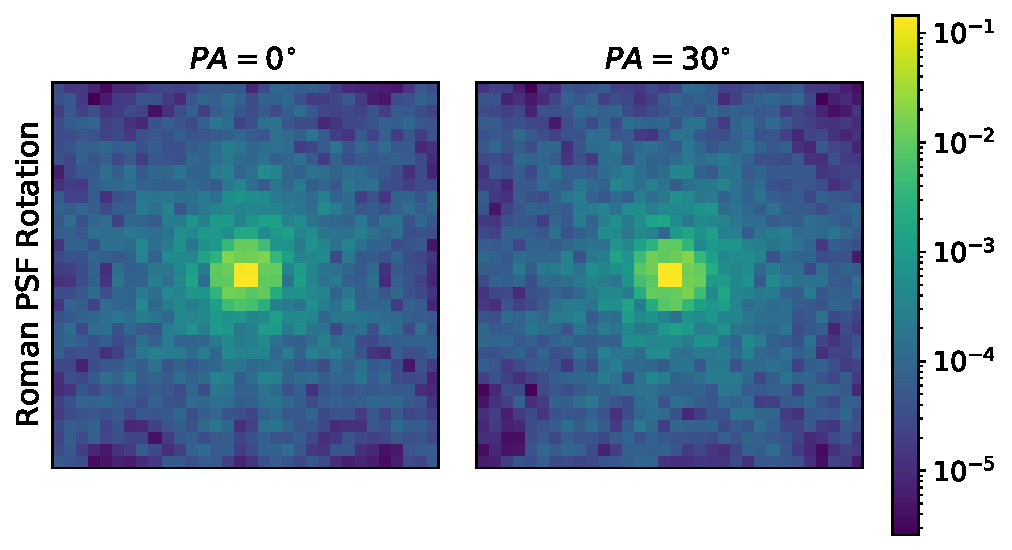
\includegraphics[width=\columnwidth]{psf_rotation.pdf}
% 	\vspace*{-3mm}
    \caption{The rotation of the Roman PSF produced by the \texttt{galsim.roman} module. The position angle (PA) which determines the rotation of the focal plane is $0^{\circ}$ and $30^{\circ}$ clockwise. These are drawn for SCA=1 and H158 bandpass at a native pixel scale. The rotation of the PSF is particularly important when an object has multiple exposures. As more exposures are rotated relative to one another on the sky, the average impact of the PSF will be rounder. This will translate to a substantially less-elliptical coadd PSF.}
    \label{fig:psfrot}
\end{figure}

\begin{figure*}
	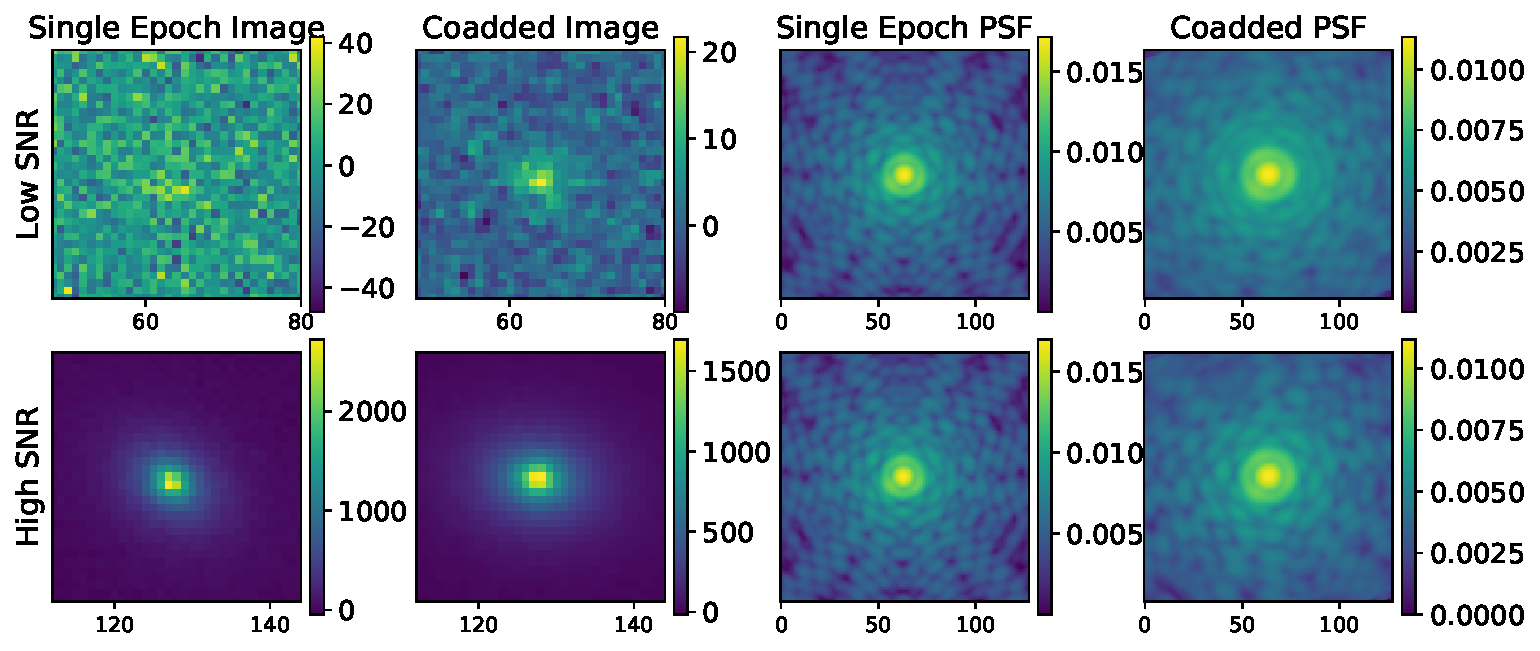
\includegraphics[width=\textwidth]{lowsnr_highsnr_galaxies.pdf}
	%\vspace*{-10mm}
    \caption{The top row shows the first observation of the single epoch images and its coadded image, and the corresponding single-epoch and coadded oversampled PSF images for a galaxy with low signal-to-noise ratio (S/N=9.69 in a single-epoch image). The bottom row shows the same for a galaxy with high signal-to-noise ratio (S/N=1552.97 in a single-epoch image). The PSFs are shown in a log-scale. The single epoch PSFs are almost identical, since there is no visually different feature for modeling them in different dithers and SCAs. Coadded PSFs look slightly different due to different numbers of single exposures. }
    \label{fig:singlecoadd}
\end{figure*}


\subsection{Updates to Simulation Capabilities}
In order to accomplish the science goals, and build and test weak lensing calibration pipelines for \emph{Roman}, we have continued to update the realism of our image simulations. We have implemented and made updates to the following parts of the simulation framework to be able to better test shear calibration using \textsc{metacalibration}. 
\begin{itemize}
    \setlength\itemsep{1em}
    \item \textbf{Saturation Cuts}:
    We have implemented a pixel saturation limit of 100,000 electrons. This value is an approximate pixel saturation level, but in the next generation of the simulations we will use a more accurate pixel saturation limit measured directly from the flight candidate detectors. 
    
    \item \textbf{Rotation of the \emph{Roman} PSF on the sky}:
    In the study by T21, the rotations of the \emph{Roman} PSF with respect to the telescope rotation were not properly applied by the \texttt{galsim.roman} module. Since a non-rotating PSF produces an artificial preferred direction, which can translate to galaxy shapes through errors in the process of deconvolvution, properly accounting for the averaging of the PSF orientation across exposures due to the survey dithering strategy is essential for a realistic shear calibration estimate. There has been an update in the \texttt{galsim.roman} module to correctly rotate the PSF given the WCS of the SCA in a given telescope pointing. Figure \ref{fig:psfrot} shows an example of how the PSF for one SCA changes with the rotation angle of the telescope.
    
    \item \textbf{Single-band and Multiband Coadds}: 
    We have used the postage stamp coadds (\texttt{psc}) algorithm\footnote{\url{https://github.com/esheldon/psc}} to create coadditions of single-epoch postage stamps of individual objects. Coadds are usually performed to enhance the signal-to-noise ratio (S/N) of an image and mitigate the impacts of measurement noise, while allowing for better sampling of the image if the overlapping images are dithered. However, it is challenging to create a robust, continuous coadd PSF model over an entire image. This is mitigated if we instead construct small, local coadds (at the size of an object postage stamp cutout in this work), which is a method also utilized in \textsc{metadetection}. If we take advantage of fitting an object in the coadd instead of fitting multiple images of each object in each filter, we can save a factor of approx. six in computing time, which is the average number of exposures from the reference survey. Additionally, coadding is one way to reduce the effect of the undersampling of the images since the coadd can be better sampled due to dithering. For these reasons, we explore utilizing a coadding scheme for the \emph{Roman} galaxies. The detailed overview of the coadd process in \texttt{psc} is described in Sec. \ref{subsec:psc}. 
    
    \item \textbf{\textsc{metacalibration} in \texttt{ngmix}}: We implemented the \textsc{metacalibration}\footnote{\url{https://github.com/esheldon/ngmix/wiki/Metacalibration}} bootstrapper method, which is a wrapper class to run measurements in the \texttt{ngmix} package and was used to produce the weak lensing shape catalog in the DES Y3 analysis (\citealt{2020arXiv201103408G}). The \textsc{metacalibration} process can be performed on single-epoch or coadd images in each bandpass. With this calibration method, we hope to significantly reduce some of the shear calibration bias T21 measured in order to make comparisons of effects contributing to the bias more realistic and meaningful as we explore future \emph{Roman} pipeline development. The detailed overview of \textsc{metacalibration} can be found in Sec.~\ref{subsec:mcal}. 
    %\item (Any other changes?)
\end{itemize}


\subsection{Validations with Simple Simulations}
\label{subsec:simplesim}
The purpose of the simple simulations is to verify that there are no systematic biases at the fundamental levels of the simulation (e.g., no complex detector effects). These simple simulations play a role in ruling out the sources of systematic biases that may potentially be a problem in the use of \textsc{metacalibration} with space-based images. 

The fixed parameters for the simulations are listed in Table. \ref{tab:params}. With these parameters, we simulated images with varying galaxy model profile, PSF model profile, the artificial shear, and background noise level, without any complications in the images and pipelines such as detector effects and coaddition. We set the basic light profiles for galaxies and PSF to be Gaussian. We first verify that our input gravitational shear is unbiased in \textsc{metacalibration} framework and the uncertainty in the recovered shape is small enough for the \emph{Roman} requirement (Fig. \ref{fig:metacal_shear_linear}). We then test the pipeline by doubling the background noise. Due to \emph{Roman} being in NIR range, the expected background noise level in the images is higher compared to optical imaging surveys like DES. With this test, we can confirm that the treatment of correlated noise induced in the  \textsc{metacalibration} process for low S/N objects does not trigger any bias at the level we should be concerned (\citealt{2017ApJ...841...24S}). Another test with \emph{Roman} PSF instead of Gaussian PSF does guarantee that the PSF features particular to \emph{Roman} do not bias the shape recovery even though it is undersampled. Upon validating there does not exist any bias at the fundamental level, we began constructing coadd and more complex measurement pipeline. 
\begin{table}
    \centering
    \begin{tabular}[width=\columnwidth]{|p{3cm}||p{3cm}|p{3cm}|p{3cm}|}
    \hline
    Parameter & Value \\
    \hline
    Pixel scale & 0.11 arcsec/pixel\\
    Dither, SCA & 22535, 1 \\ 
    Bandpass & H158 \\
    Half-light radius & 1.0 arcsec\\
    Magnitude & randomly chosen from \emph{CANDELS} \\ 
    Stamp size & 32 pixels each side\\
    \hline
    \end{tabular}
    \caption{List of the parameter choices for the simple simulations.}
    \label{tab:params}
\end{table}

\begin{table*}
	\centering
	\label{tab:simple_sim}
	\begin{tabular}[width=\textwidth]{ c|c|c|c|c|c|c|c|c|c } 
		\hline
		simulation variants & galaxy profile & PSF profile & shear & background noise level & $m_{1}\times10^{-2}$ & $m_{2}\times10^{-2}$ & $c_{1}\times10^{-4}$ & $c_{2}\times10^{-4}$\\
		\hline
		Basic-0.02 & Gaussian & Gaussian & 0.02 & roman.getSkyLevel & 0.01$\pm$0.10 & -0.02$\pm$0.10 & -0.02$\pm$0.14 & 1.06$\pm$0.14\\
		Basic-0.05 & Gaussian & Gaussian & 0.05 & roman.getSkyLevel & 0.23$\pm$0.07 & 0.22$\pm$0.07 & 0.05$\pm$0.33 & 1.08$\pm$0.33\\
		Basic-0.1 & Gaussian & Gaussian & 0.1 & roman.getSkyLevel & 0.99$\pm$0.03 & 0.99$\pm$0.03 & 0.13$\pm$0.33 & 0.88$\pm$0.33\\
		\hline
		Doublesky-0.02 & Gaussian & Gaussian & 0.02 & 2 $\times$ roman.getSkyLevel & -0.12$\pm$0.18 & 0.01$\pm$0.18 & 0.06$\pm$0.36 & 1.04$\pm$0.36\\
		\hline
		RomanPSF-0.02 (non-rotated) & Gaussian & Roman & 0.02 & roman.getSkyLevel & 0.13$\pm$0.10 & 0.18$\pm$0.10 & -0.02$\pm$0.19 & 5.33$\pm$0.19\\
		\hline
	\end{tabular}
	\caption{This table compares the shear calibration bias, both multiplicative and additive bias for different simulation runs.}
	\label{tab:result}
\end{table*}

\begin{figure}
	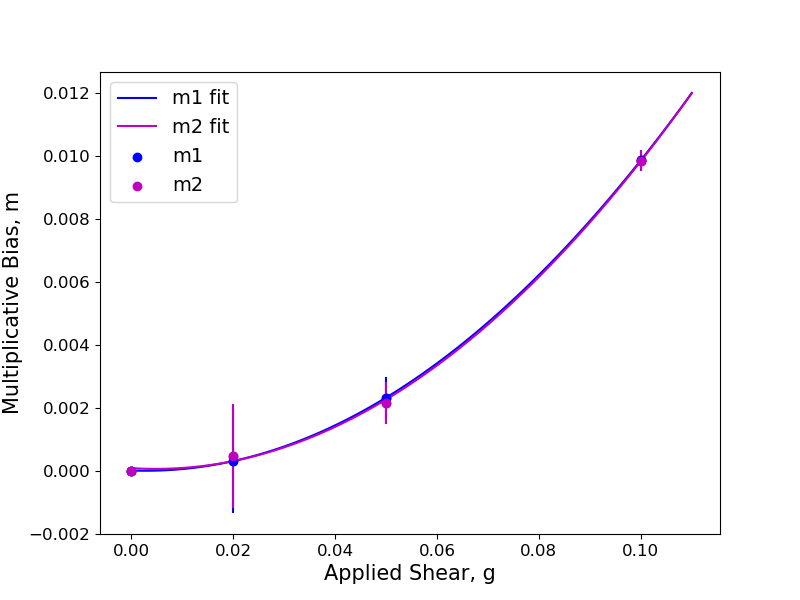
\includegraphics[width=\columnwidth]{metacal_bias_shear.png}
    %\vspace*{-5mm}
    \caption{We show the recovered multiplicative bias on the shear as a function of applied shear for the choice of the applied shear in our simulations. At first order, the \textsc{metacalibration} method only works for small shears. The next order effect is seen as a quadratic dependence of the multiplicative shear bias on the applied shear. A larger input shear increases the signal-to-noise of bias estimates, but to keep the non-linear effect small compared to requirements, we limit input shears to $\pm 0.01$.}
    \label{fig:metacal_shear_linear}
\end{figure}


\section{Coadd and shear calibration pipelines}
\label{sec:methods}
Our goal is to test whether the recovered shapes with \textsc{metacalibration} are non-biased for \emph{Roman} and to understand the factors that might contribute to any non-negligible bias. In order to do so, we need to build a measurement pipeline within the current simulation framework that produces a final calibrated shear measurement. In this section, we present in detail how coadd images are produced with \texttt{psc} from the undersampled single-epoch images and how \textsc{metacalibration} is implemented to calibrate the measured shear using the \textsc{metacalibration} catalog. 


\subsection{Postage Stamp Coadds}
\label{subsec:psc}
Coaddition is the process of summing information from multiple overlapping images. If the single-epoch images are dithered, a Nyquist-sampled image can be constructed out of multiple exposures of an object. While this process can also be beneficial in increasing the S/N value of an object and reducing the impact of pixel noise, several challenges need to be addressed for images taken with telescopes that can rotate. When rotation is introduced, this coadding process becomes more complex to interpolate the image to stack a pixel grid. While coaddition can introduce new challenges and potential biases due to the complexity of coadding the original PSF and its interpolation scheme, the bias due to the undersampling of the original images can be mitigated by appropriately coadding dithered images. (choice of psc? -> to avoid thinking about rotations of the whole image, coadding cutouts is much easier. )

We reconstruct a better-sampled coadd image from multiple exposures in MEDS files. For the coaddition of the PSF, we choose to coadd the image with an oversampled PSF `model'. We oversample the original PSF by a factor of 4 to simulate the better sampled PSF model that will eventually be possible to construct during the \emph{Roman} mission. For each exposure of the object we render the \emph{Roman} PSF with a stamp size of 32 pixels at the galaxy centroid. We modified the original \texttt{psc} code to improve performance for this \emph{Roman} study, and these modifications are listed below with the general coadding process in \texttt{psc}. 

The algorithm: 
\begin{enumerate}
    \setlength\itemsep{1em}
    \item Finds the wcs of the first exposure of the object.
    \item Translates the original wcs to a flat wcs, because it produces more stable results with \texttt{ngmix}.
    \item Creates the coadd stamp with 0.8 $\times$ original pixel scale. We scale the original pixel scale of the final coadd stamp to mitigate the effect of undersampling. This final pixel scale was chosen to prevent the presence of visual artifacts in the structure of the coadd PSF image. 
    \item Creates an interpolated image with \texttt{GalSim} with the object centroid appropriately offset for each image using a \texttt{lanczos3} interpolation method and sums them. Out of several interpolation methods we tried, \texttt{lanczos3} produced the best coadd of the PSF.
    \item Creates a coadded noise image from the weight of the original images. 
\end{enumerate}
Figure \ref{fig:singlecoadd} shows an example of the simulated single-epoch and coadded images and PSFs for objects with low and high S/N. Note that the shape and struts pattern in the original PSF can be washed out by coadding the rotationally dithered PSFs. 


Before we measure and calibrate shapes with \texttt{ngmix}, we downsample the high-resolution PSF to the original pixel size. Figure \ref{fig:coadd_oversample_res} shows the coadded oversampled PSF and the then-downsampled PSF, and their differences. Having a matching pixel scale in the galaxy and PSF image is a requirement for the current \texttt{ngmix} pipeline. Future versions of these measurements should include the ability to provide a better-sampled PSF image for deconvolution in the measurement. Figure \ref{fig:single_to_coadd_rgb} shows the coadd products in different bandpasses for a relatively high S/N object. The multiband PSF image is the oversampled version for better visualization. 


\begin{figure}
	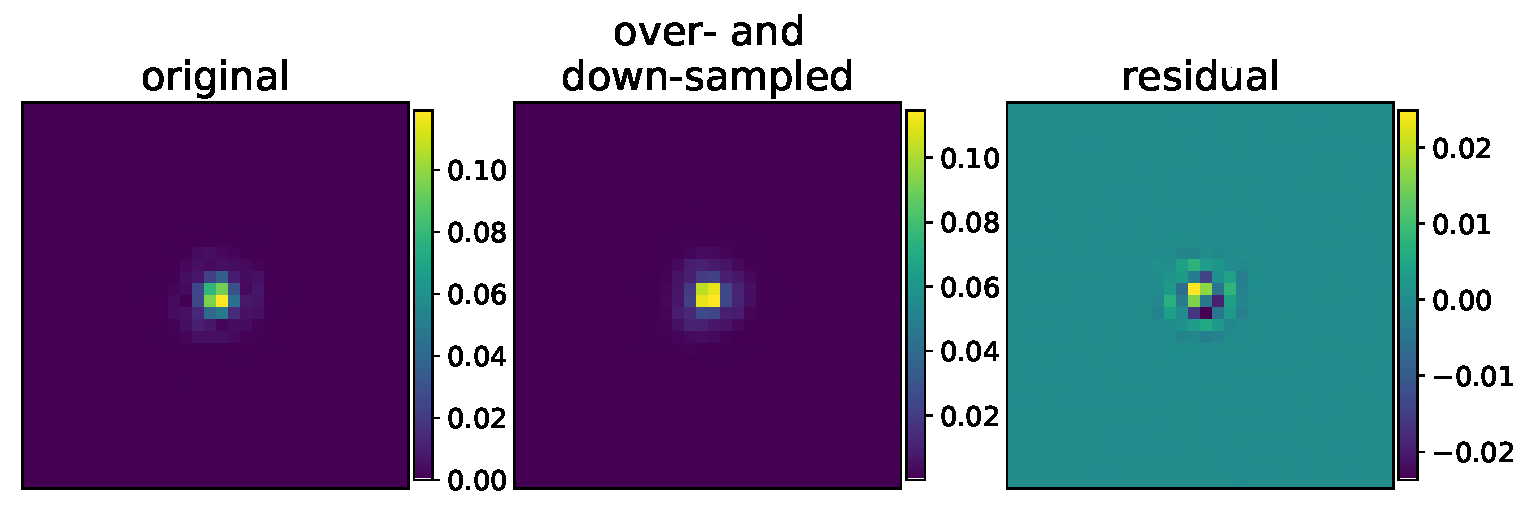
\includegraphics[width=\columnwidth]{psf_differences_v2.pdf}
    % \vspace*{-5mm}
    \caption{The left and middle panels illustrate the coadded \emph{Roman} PSF at its original pixel scale and the coadded PSF with a pixel scale that is generated with a pixel scale that is smaller by a factor of 4 and then downsampled to this original pixel scale. These are visualized on a log scale. The right panel shows the difference image between the two PSF images. }
    \label{fig:coadd_oversample_res}
\end{figure}


\begin{figure*}
	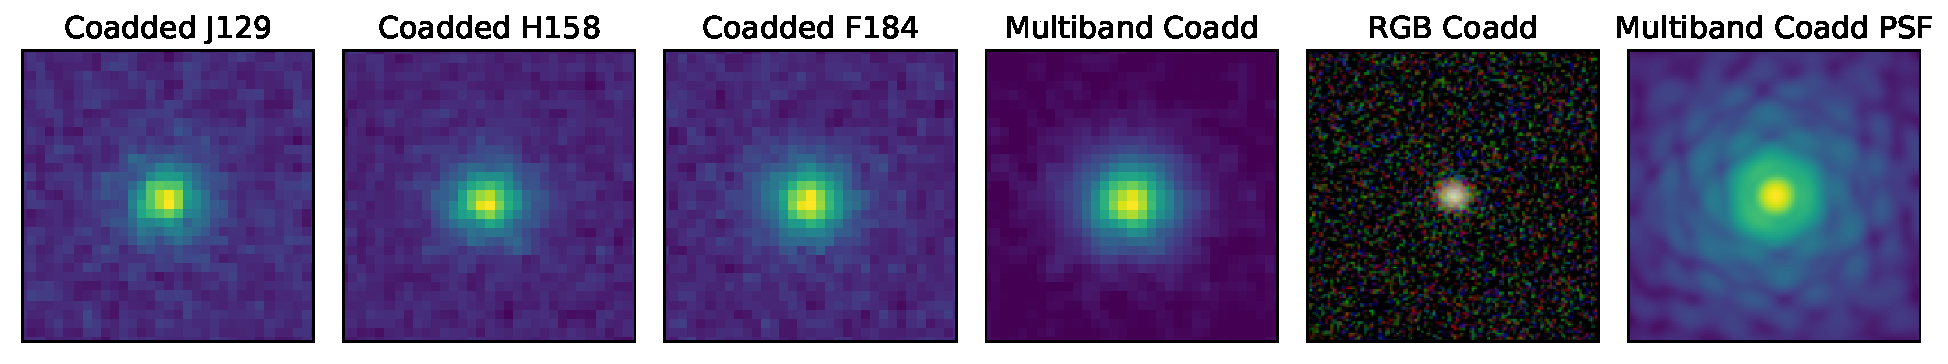
\includegraphics[width=\textwidth]{coadd_galaxy_example_log.pdf}
    %\vspace*{-20mm}
    \caption{The left 3 panels show an example of the coadded galaxy images for each filter. The S/N for each filter is S/N=90, 68, 108, respectively. The 4th and 5th panels show the multiband coadd images of the same object; each with linear scale and RGB scale. The S/N of the coadd image is S/N=110. Finally, the right-most panel shows the coadded oversampled PSF on a log scale.}
    \label{fig:single_to_coadd_rgb}
\end{figure*}

\par

\subsection{Shape Calibration \& Measurement with \texttt{ngmix}}
\label{subsec:mcal}
Once we construct the individual galaxy stamp coadds from the MEDS files, we recover the calibrated shear signal using the \textsc{metacalibration} process (\citealt{2017arXiv170202600H, 2017ApJ...841...24S}). The bootstrapper method used in \texttt{ngmix} wraps the \textsc{metacalibration} and the shape fit processes. The priors needed for the fit are listed in Table \ref{tab:priors}. We note that we have run \textsc{metacalibration} with \texttt{fitgauss} and \texttt{gauss} parameters for the new PSF model, and we found that the \texttt{gauss} method performs better for our case.

\begin{table}
    \centering
    \begin{tabular}{|p{3cm}||p{3cm}|p{3cm}|p{3cm}|}
    \hline
    Prior & Value \\
    \hline
    Pixel centroid offset & 0 < $p_{x,y}$ < 0.11\\
    Shear & $|g|=1.0$, $\sigma_{|g|} = 0.3$\\
    Half-light radius & $10^{-5}$ < T < $10^{4}$\\
    Flux fraction of the bulge  & $\langle f\rangle = 0.5$, $\sigma_{f} = 0.1$\\
    Total flux & $0$ < F < $10^{6}$\\
    \hline
    \end{tabular}
    \caption{List of prior values used for the Gaussian mixture fit.}
    \label{tab:priors}
\end{table}

\textsc{metacalibration} creates one unsheared and four artificially-sheared galaxy stamps. Each is deconvolved with the input PSF, left unsheared or sheared with an additional gravitational shear of $\delta\gamma=\pm 0.01$ in the two basis directions ($+g1$, $-g1$, $+g2$, $-g2$) and re-convolved with a new slightly larger isotropic, Gaussian PSF. \textsc{metacalibration} works under the assumption that the input shear is small, otherwise the recovered shear would be biased without accounting for higher order terms. It is a balance to choose an input shear that results in higher S/N of an object and unbiased shape measurement. Figure \ref{fig:metacal_shear_linear} shows the performance as a function of input shear leading to the choice of input shear $\gamma=\pm 0.02$. 

After processing the images in \textsc{metacalibration} and measuring the shapes in \texttt{ngmix}, we have 5 shape catalogs in each \textsc{metacalibration} shear direction. We can then compute the shear response from these catalogs and calculate the calibrated ensemble galaxy ellipticities. The shear response can be understood as the change in objects' ellipticities with respect to the change in gravitational shear. Mathematically, the observed ellipticities, $\vb*{e}$ = ($e_{1}$, $e_{2}$), can be approximated using a Taylor expansion around the two-component shear, $\vb*{\gamma}=0$. Higher terms here can be dropped assuming the gravitational shear is small. 
\begin{equation}
    \vb*{e} = \vb*{e}\rvert_{\vb*{\gamma}=0} + \frac{\partial \vb*{e}}{\partial \vb*{\gamma}}\bigg\rvert_{\vb*{\gamma}=0}\vb*{\gamma} + \ldots
\end{equation}
From this expression, the shear response matrix can be defined as, 
\begin{equation}
    \vb*{R} \equiv \frac{\partial \vb*{e}}{\partial \vb*{\gamma}}\bigg\rvert_{\vb*{\gamma}=0} = 
    \begin{pmatrix}
        \partial e_{1}/\partial \gamma_{1} & \partial e_{2}/\partial \gamma_{1} \\ 
        \partial e_{1}/\partial \gamma_{2} & \partial e_{2}/\partial \gamma_{2}
    \end{pmatrix}. 
\end{equation}
The ensemble mean of measured ellipticities $\langle\vb*{e}\rangle$ can then computed. Since we expect galaxies to be randomly oriented such that $\langle\vb*{e}\rangle\rvert_{\vb*{\gamma}=0}=0$, we have a relationship between the measured ellipticities and the input shear in the simulations, 
\begin{equation}
    \langle\vb*{e}\rangle \approx \langle \vb*{R}\vb*{\gamma} \rangle. 
\end{equation} 


In practice, we compute the mean shear response from the five versions of \textsc{metacalibration} catalog using the finite difference method. 

\begin{equation}
    \langle\vb*{R_{ij}}\rangle = 
    \frac{\langle e^{+}_{i} - e^{-}_{i} \rangle}{\delta\gamma_{j}}, 
\end{equation}
where $e^{+}_{i}$ and $e^{-}_{i}$ is the $i$-th component of the galaxy ellipticity where positive ($+$) or negative ($-$) shear is applied in $i$-th direction. 


Then, this shear response is used to compute the multiplicative ($\vb*{M}$) and additive ($\vb*{C}$) bias using the linear shear bias model (\ref{eqn:linear}). The covariances are computed using the bootstrap estimate of standard error. From the observed ellipticity catalogs, we randomly choose $n$ samples with replacement which is the length of the data set, and compute the distributions of multiplicative ($f^{M}_{i}$) and additive ($f^{C}_{i}$) bias for $i=1,2,3,...,N$ in the same way as above. The distributions are then used to compute the error estimate,  


\begin{equation}
    \sigma_{N,f} = \sqrt{\frac{1}{N-1} \sum_{i=1}^{N}(f_{i}-\bar{f_{i}})^{2}}, 
\end{equation}
where we use sample $N$=200.  \textcolor{red}{is it the same if you do jackknife?}


\section{Results}
\label{sec:results}
In this section, we present the properties of the simulated data products and the shape measurement results from various simulation variants. We divide our shape measurement into two categories; single-band and multiband. For single-band measurements, in each filter, we measure the shapes from the original single exposures by jointly fitting them. We set our base case to be this single-band joint-fit measurement. As the more developed case, we measure shapes with the single-band coadd in each filter. For the single-epoch multiband measurement, we match the objects between each filter and measure the shapes with the joint-fit of single exposures across all the filters. The coadd multiband measurement is jointly fit across the three coadds from each filter to recover the shapes. 

\subsection{Statistics of the Shape Catalog}
From the CANDELS catalog, based on the \emph{Roman} Weak Lensing mission requirements, objects are pre-selected and simulated. In total, the galaxy photometry catalog contains 907,170 galaxies and from this catalog we simulated galaxies on 18 SCAs across 198 pointings for F184, 227 pointings for H158, and 238 pointings for J129 bandpass. We do not make any selection cuts on the simulated catalogs based on measured properties, since all input objects should pass requirements for weak lensing selection (e.g., S/N>18). Even so, due to the misestimation of the PSF or low S/N, the Gaussian mixture in \texttt{ngmix} fails to fit about 5\% of all simulated objects, and so the total number of the recovered objects for single-band measurements is, 861,407 for F184, 863,146 for H158, and 859,193 for J129. For the multiband (H158+J129+F184) coadd measurements, we use objects that are measured successfully in all of the filters and the total number of the recovered objects is 851,821.
Figures \ref{fig:true_properties} and \ref{fig:measured_properties} show the true properties from the truth catalog and measured properties from the \textsc{metacalibration} shape catalogs. 

\begin{figure}
	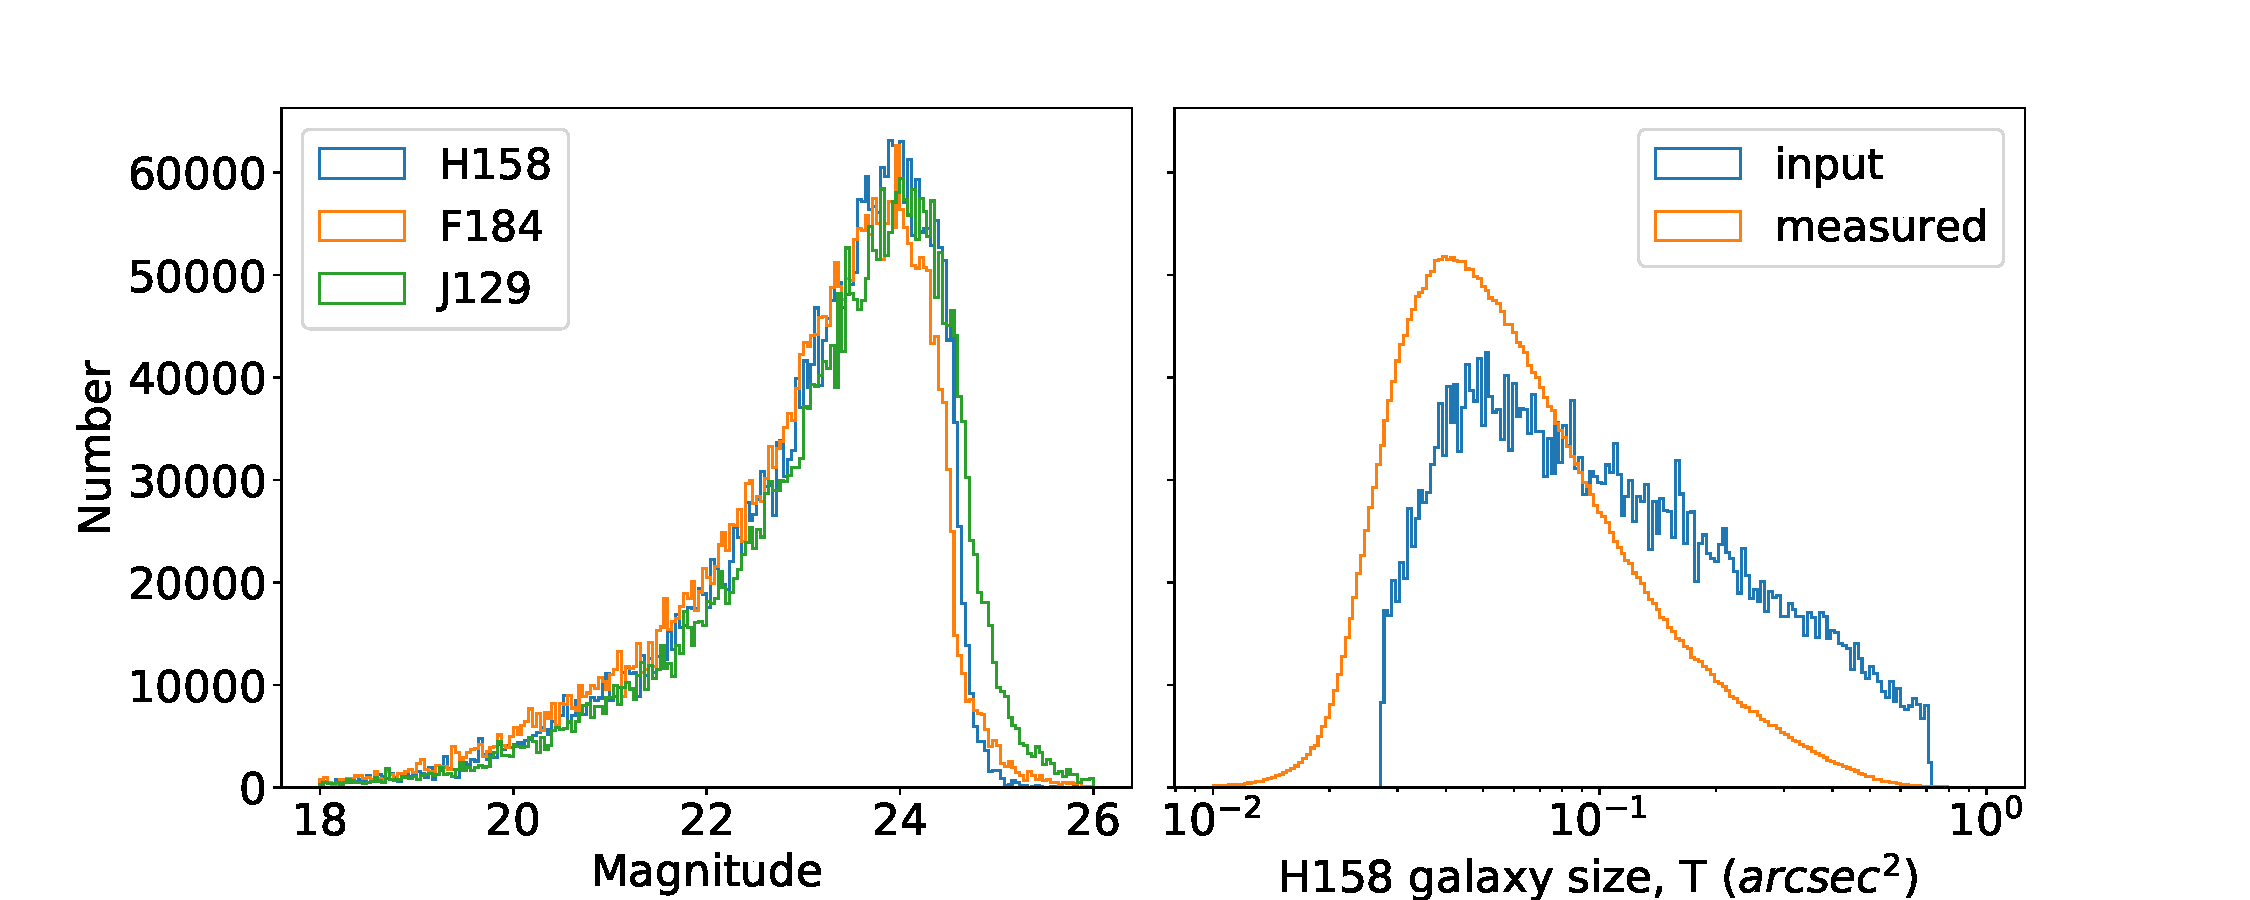
\includegraphics[width=\columnwidth]{true_properties.pdf}
	\centering
    \caption{The left panel shows the measured magnitudes of galaxies for  the 3 filters we have used to measure shapes. The mean magnitude for H158, F184, and J129 are respectively 23.098, 22.976, and 23.273. The right panel shows the half-light radius in units of arcsec for H158 for input and measured objects. The mean half-light radii for input and measured galaxies are 0.294 and 0.221 arcsec for H158.}
    \label{fig:true_properties}
\end{figure}

\begin{figure*}
    %\hspace*{-3.1cm}
    \centering
	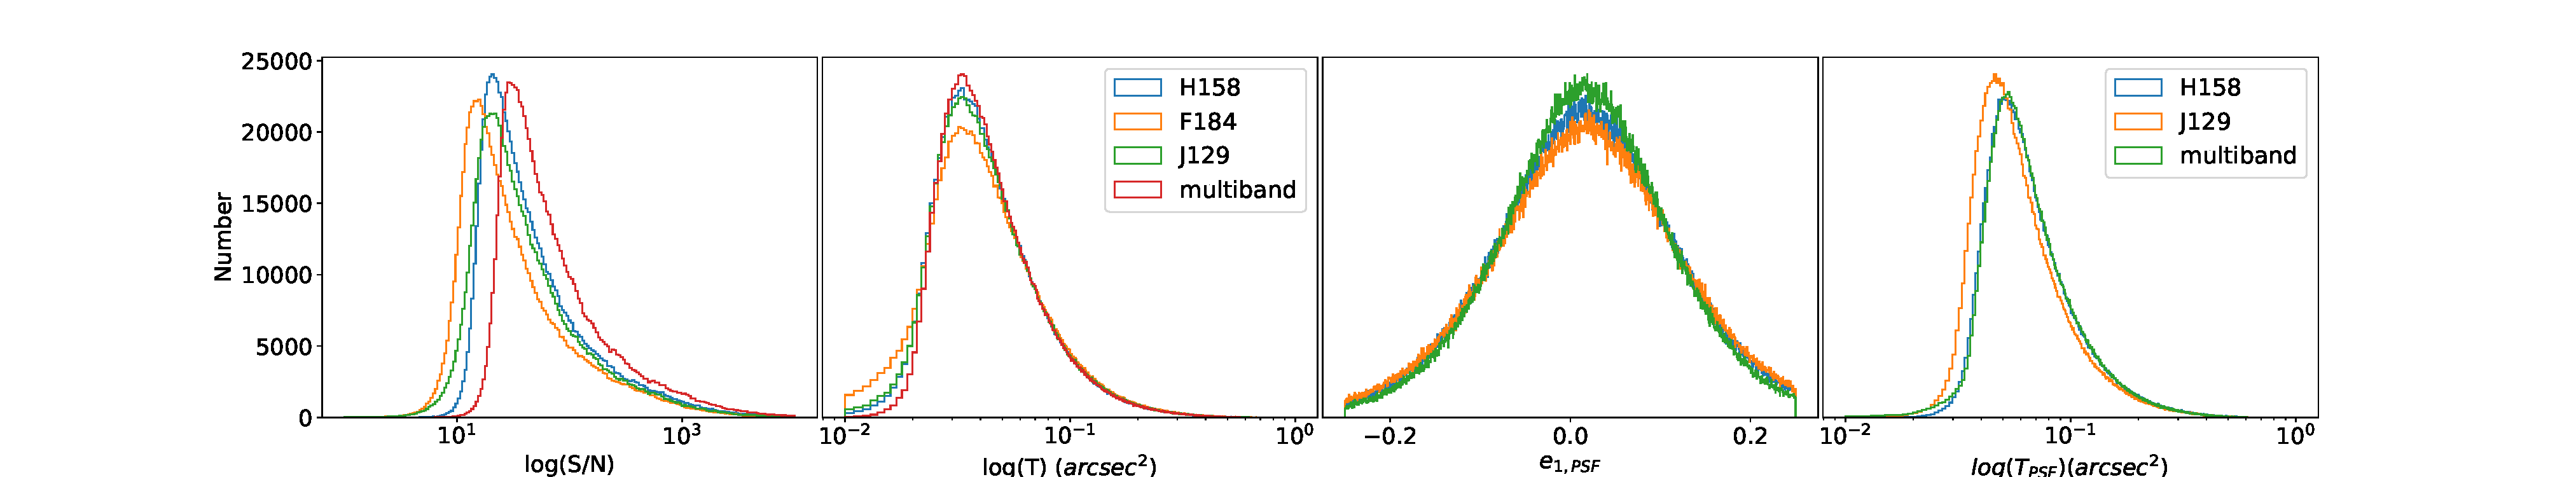
\includegraphics[width=\textwidth]{ngmix_snr_T.pdf}
    \caption{The histograms of measured galaxy and PSF properties in \texttt{ngmix} for single-band coadd and multiband coadd measurements. It includes S/N, galaxy size $T{gal}$, and the shape and size of the PSF. The S/N is significantly improved in the multiband fit.}
    \label{fig:measured_properties}
\end{figure*}


\subsection{Shear Calibration Bias}
\label{subsec:shapes}
We estimate the levels of shear calibration bias associated with calibrating shapes with \textsc{metacalibration} in \emph{Roman} images as described in Sec. \ref{subsec:mcal}. The multiplicative and additive bias values listed in the text are the average of $m_{1}$ and $m_{2}$, and $c_{1}$ and $c_{2}$. These are usually symmetric, except in the case of the coadd measurements, where $c_1>c_2$. The comprehensive results can be found in Table \ref{tab:bias_summary} and the single-band coadd result compared to the previously measured values in Fig. \ref{fig:final_result}.  

For the single-band measurements, we can use the sampling factor defined in Equation \ref{eqn:sampling} per bandpass to show the relationship between the shear bias and image sampling. The sampling factor is an indication of how undersampled the image in some bandpass is. The sampling factor for each single-band measurement can be found in Table \ref{tab:bias_summary}. This relationship between sampling factor and shear bias was previously explored in \citealt{2021MNRAS.502.4048K} using \emph{Euclid} simulation with different shape measurement algorithms, where they found that the estimated multiplicative bias has a relatively large dependence on the sampling factor. Their result can be extrapolated to our single-band single-epoch results. The multiplicative bias of single-band single-epoch measurements is roughly 1\% in each filter. When the coadded images for each filter are used, the bias is at a similar level or worse within the uncertainties. We can conclude that in the current \emph{Roman} simulation the multiplicative bias has a similar dependence on the sampling factor as shown in K21, but with a smaller amplitude. We do not see any clear improvements in the recovered shear when we coadd the single-epoch images, despite having a smaller pixel scale (better sampling) in the images. This is most likely due to an issue with how we are currently treating the PSF or correlated noise in the coadding process, given the large observed $c_1$ when coadding discussed below. \textcolor{red}{Although we have verified that the handling of correlated noise in \textsc{metacalibration} proess for single-epoch images is unbiased, it is possible that the \texttt{psc} process induces more correlated noise that is not corrected further. }

The additive bias of the single-band single-epochs measurements for each filter is smaller about an order of magnitude than that of the coadd measurements. The estimated additive bias is the same order as that found in the Y3 analysis in DES, which uses a similar shear calibration pipeline. In Table \ref{tab:result}, it is worth noting that the coadd process clearly introduces non-trivial additive biases in one direction of the shear, but not the other. This is due to the effect of an imperfect coadd PSF model. We find this correlation in Figure \ref{fig:meanshear} where the recovered shear on the coadd images has a strong linear dependence on the PSF ellipticity measured by an adaptive moments method (\citealt{2003MNRAS.343..459H}). The impact of the PSF shape and size leakage in the estimated galaxy shapes at the correlation function level can be estimated by computing $\rho$-statistics (\citealt{2008A&A...484...67P, 2010MNRAS.404..350R, 2016MNRAS.460.2245J}). However, we do not explore the $\rho$-statistics for our PSF model since there is no realistic shear field in this version of the simulations. We can explore these effects further in the next generation of simulations that are being worked on in parallel, which are commented on in Sec. \ref{sec:discussion}. We are also developing a more sophisticated coadd treatment that will be applied to future simulation versions and may alleviate these issues.

Finally, we discuss the results with multiband measurements. We performed multiband measurements with the three filters used in the previous measurements. One multiband measurement used all of the single epoch images from all the filters and jointly fit the shape of the galaxy. The multiplicative and additive bias is, respectively, $m=(-1.34\pm0.67)$ per cent and $c=(2.58\pm1.26)10^{-4}$. This result generally agrees with the single-band single-epochs measurements, and is consistent with zero bias at the approx. 2$\sigma$ level. We can't conclude more than that this result may be acceptable without significantly larger simulation volume of about 2000 $deg^{2}$. The other measurement is performed as a joint-fit across the coadd images for each filter. The multiplicative and additive bias is, respectively, $m=(-2.33\pm0.64)$ per cent and $c=(9.47\pm1.16)10^{-4}$. Figure \ref{fig:meanshear} shows the relationship between the mean shear and several input and measured properties of galaxies and PSF for all the measurement cases. We find that the mean shear has a linear trend as a function of input galaxy size, though the effect is one order of magnitude smaller than the mean signal.


\begin{table*}
	\centering
	\label{tab:bias_summary}
	\begin{tabular}[width=\textwidth]{ c|c|c|c|c|c } 
		\hline
		simulation variants & sampling factor ($Q$) & $m_{1}\times10^{-2}$ & $m_{2}\times10^{-2}$ & $c_{1}\times10^{-4}$ & $c_{2}\times10^{-4}$\\
		\hline
		single-epochs (J129) & 0.88 & 1.17$\pm$0.68 & 0.44$\pm$0.75 & 4.46$\pm$1.32 & 0.64$\pm$1.31\\
		single-epochs (H158) & 1.08 & -1.07$\pm$0.62 & -1.61$\pm$0.66 & 2.83$\pm$1.35 & 2.33$\pm$1.22\\
		single-epochs (F184) & 1.31 & -0.86$\pm$0.72 & -0.69$\pm$0.83 & 2.62$\pm$1.56 & 0.23$\pm$1.53\\
		\hline
		single-band coadd (J129) & 1.10 & -1.84$\pm$0.71 & -1.90$\pm$0.65 & 11.99$\pm$1.39 & 0.59$\pm$1.41\\
		single-band coadd (H158) & 1.35 & -1.75$\pm$0.67 & -1.68$\pm$0.64 & 14.39$\pm$1.32 & 4.29$\pm$1.35\\
		single-band coadd (F184) & 1.64 & -0.28$\pm$0.83 & -0.27$\pm$0.78 & 12.15$\pm$1.56 & 5.66$\pm$1.56\\
		\hline
		multiband single-epochs & N/A & -1.07$\pm$0.66 & -1.61$\pm$0.67 & 2.83$\pm$1.30 & 2.33$\pm$1.22 \\
		multiband coadd & N/A & -2.32$\pm$0.64 & -2.34$\pm$0.63 & 14.45$\pm$1.10 & 4.49$\pm$1.22\\
		
		\hline
	\end{tabular}
	\caption{This table compares the shear calibration bias, both multiplicative and additive bias for different simulation runs.}
	\label{tab:result}
\end{table*}

\begin{figure*}
	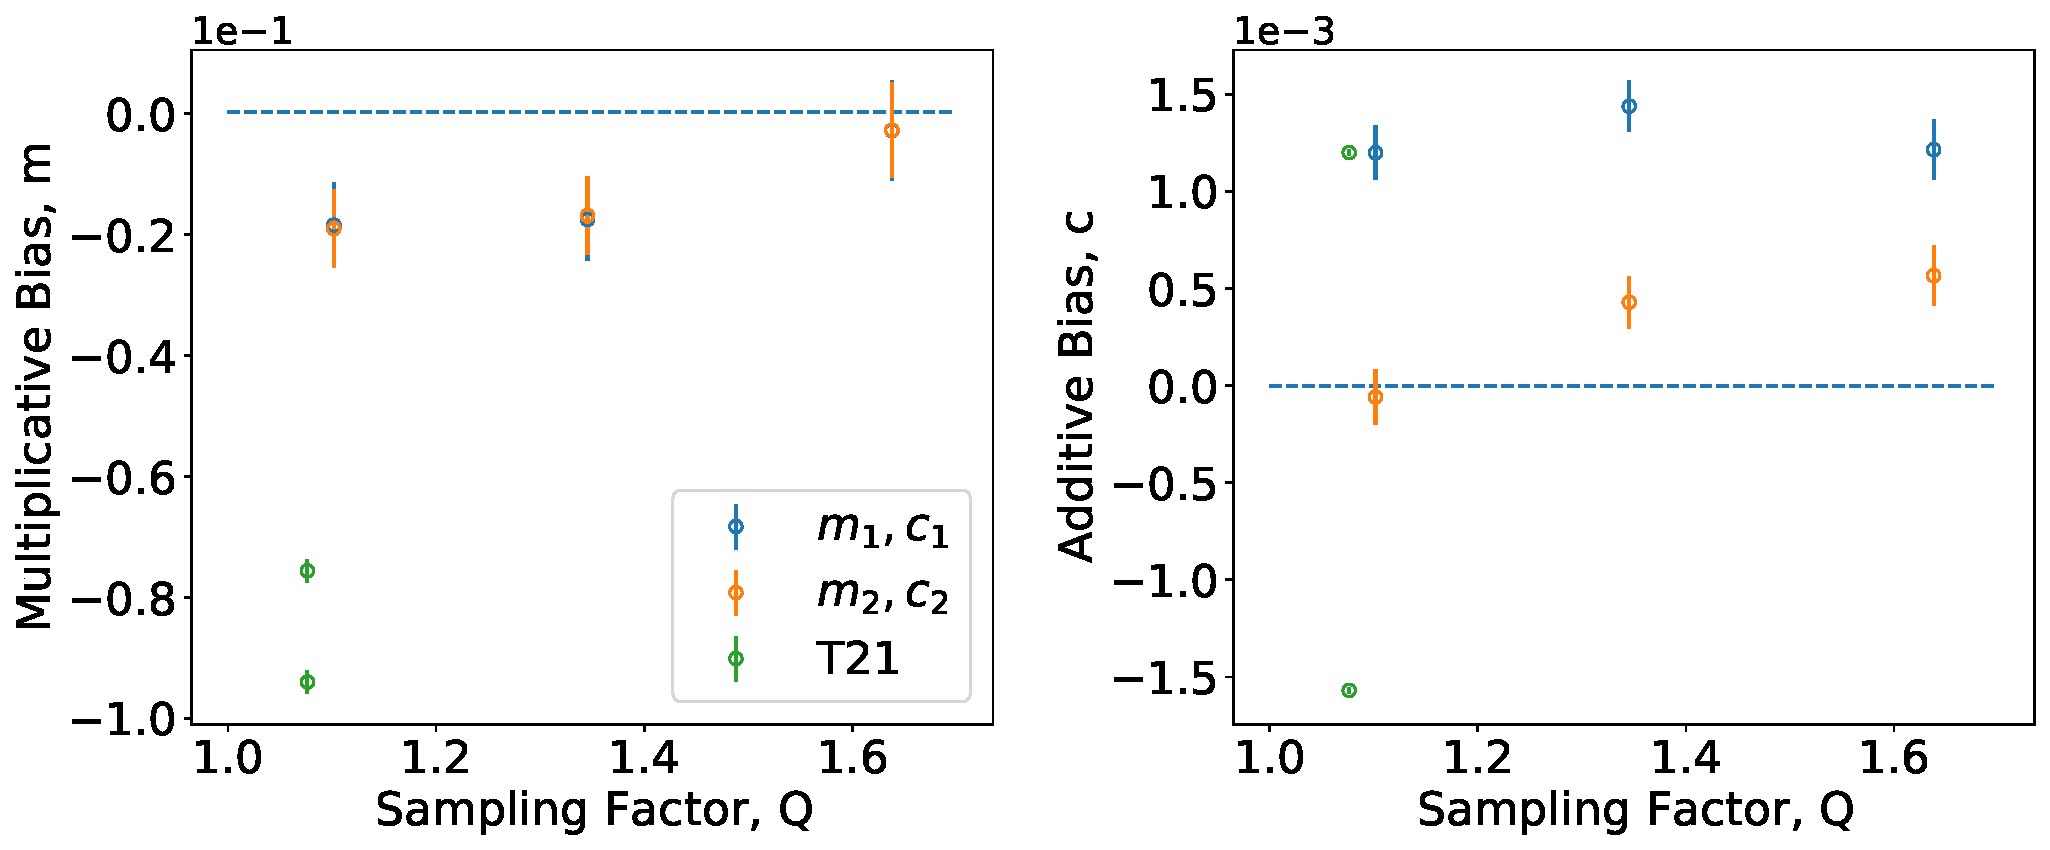
\includegraphics[width=\textwidth]{final_result_v2.pdf}
    \caption{The multiplicative ($m$) and additive ($c$) bias of the single-band coadd measurements. From left data point to the right, they represent each data for J129, H158, F184 bandpasses. T21 refers the non-calibrated result from the first-generation of the simulations by \cite{2021MNRAS.501.2044T}. }
    \label{fig:final_result}
\end{figure*}

\begin{figure*}
    %\hspace*{-3.5cm}
    \centering
	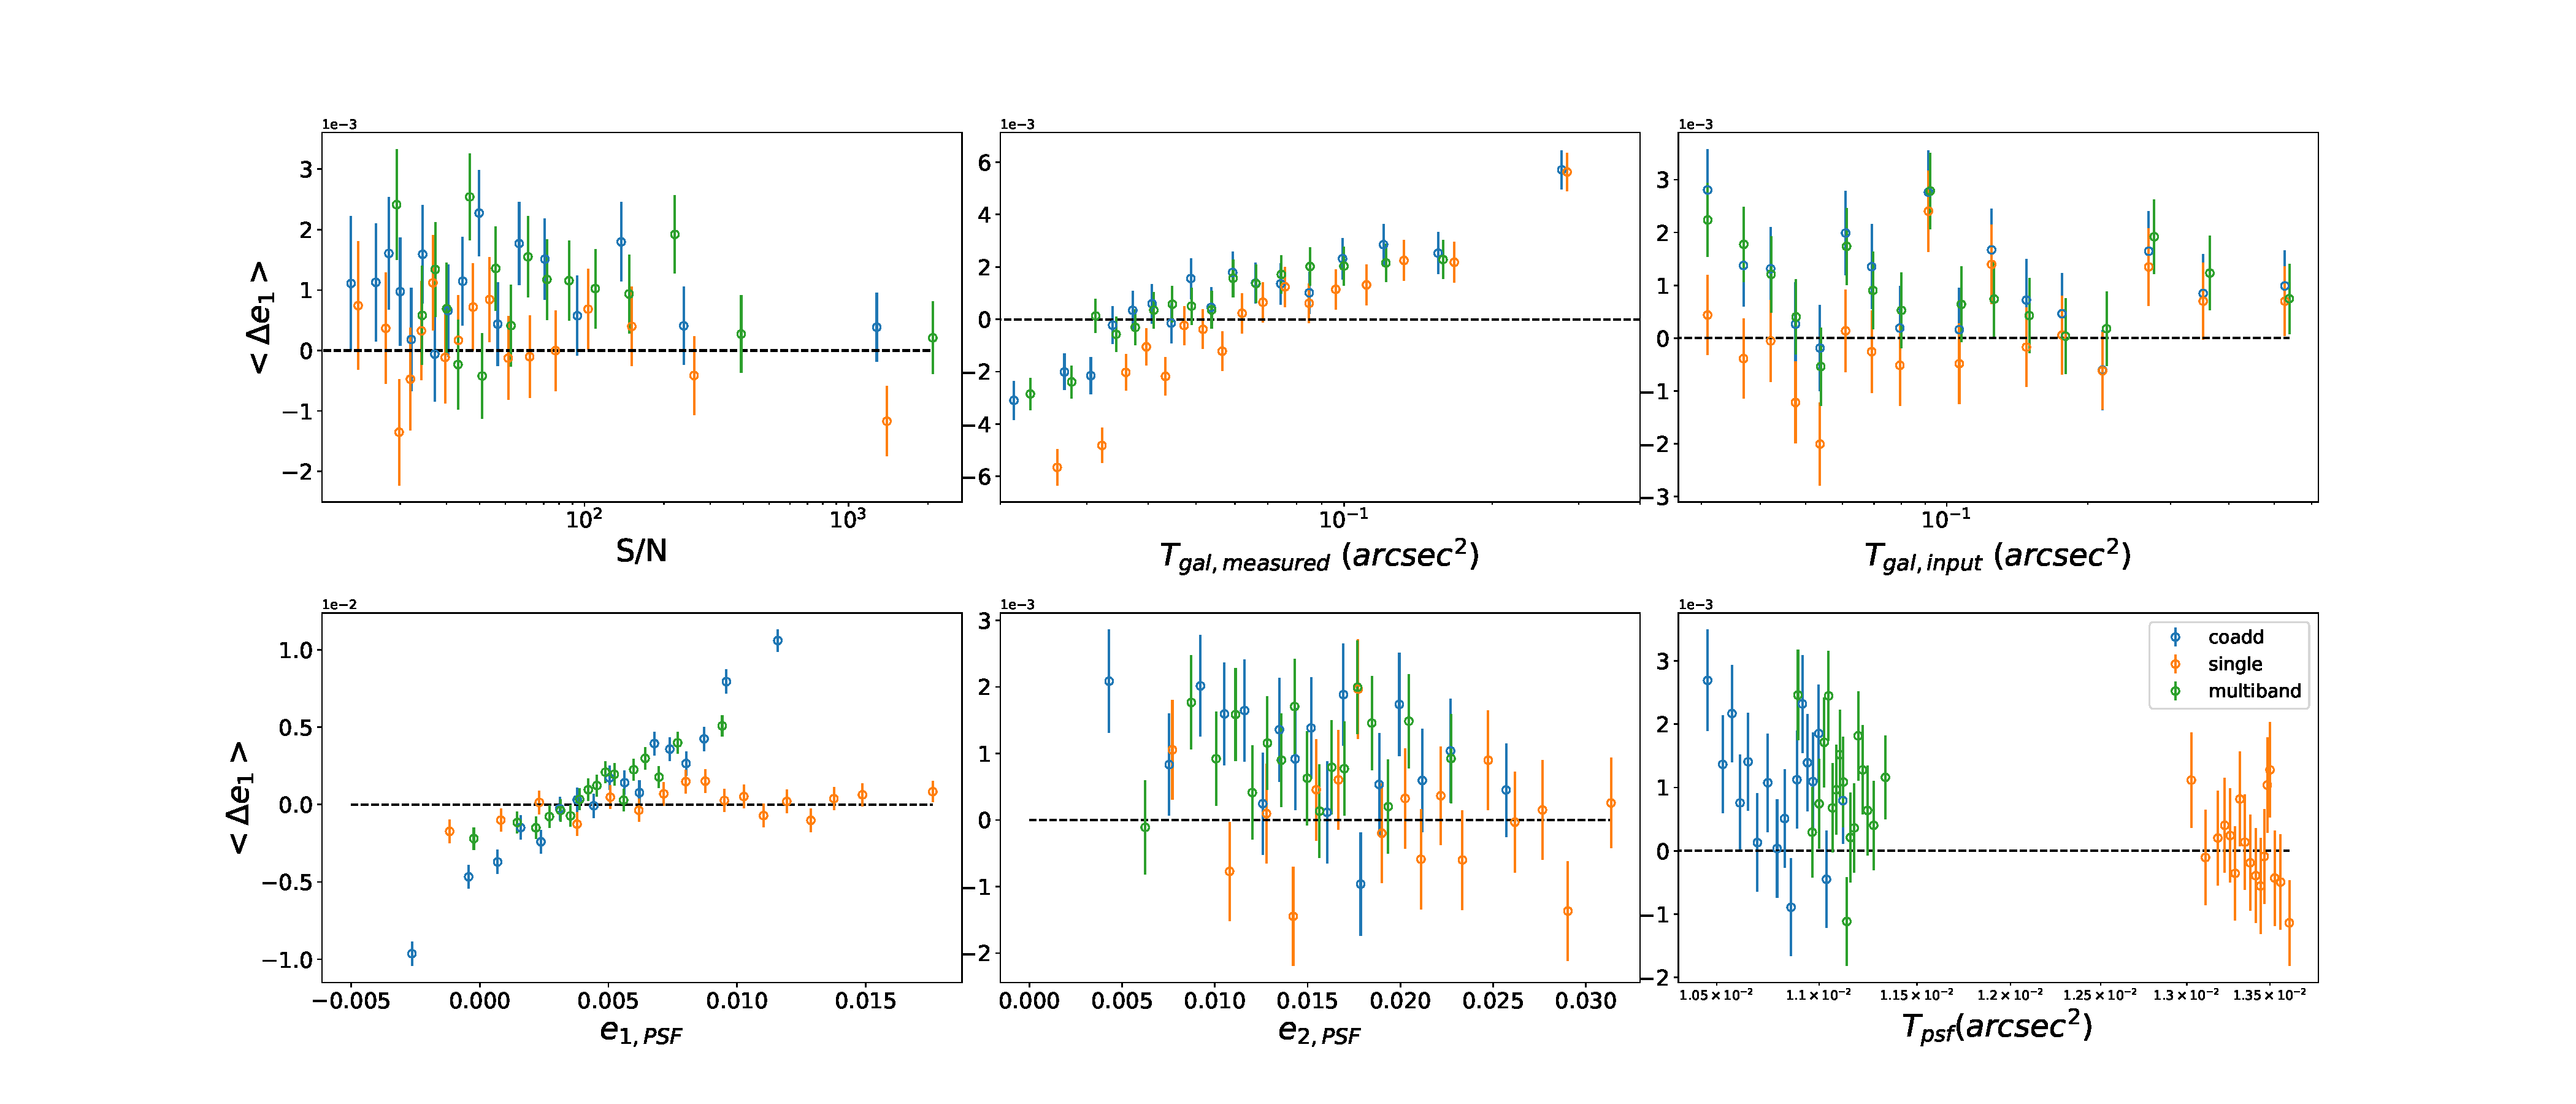
\includegraphics[width=\textwidth]{H158_meanshear_measured_properties_perbin_e1_v2.pdf}
    \caption{(Working on fixing the figure bounds)This shows the mean shear residual ($\Delta e_{1}$; $\langle e_{1,measured} \rangle - \langle e_{1,expected} \rangle$) as a function of various properties of galaxies for H158 single-band single-epochs, coadds, and multiband measurements. In this plot, the shear response is computed in each bin. The properties include the S/N, measured galaxy size $T_{gal,measured}$, input galaxy size $T_{gal,input}$, the shape and size of the input PSF.}
    \label{fig:meanshear}
\end{figure*}


\section{Future simulation needs and plan}
\label{sec:discussion}

We have investigated how \textsc{metacalibration} handles the relatively undersampled \emph{Roman} images without accounting for the effect of blending. However, it has been found that galaxy blending at different redshifts could introduce a significant shear-dependent detection bias when calibrated with \textsc{metacalibration} (e.g., \citealt{2020ApJ...902..138S}, \citealt{2020arXiv201208567M}). In future studies, we will investigate the impact of blending in Roman image simulations and implement an extended pipeline to correct shear-dependent blending/detection biases (e.g.,  \textsc{metadetection}) to explore more realistic shear calibration for the real survey. 

We have also found our postage-stamp coadd pipeline may be contributing to bias in the shear measurement, even while mitigating the effect of undersampling in the images.  This may be related to either how the undersampled PSF is treated or correlated noise effects from the simulated detector physics in the simulation. Running \textsc{metacalirbation} on simpler simulations without complex PSF shapes or detector effects showed no indication of residual bias at the level we see in the coadd shear calibration estimate. Correcting these algorithmic issues is beyond the scope of the current work, and will require a new set of improved simulations and coadd/measurement pipelines. It may also require modifications to the \textsc{metacalibration} or \textsc{metadetection} algorithms, which were constructed primarily for ground-based data, so the current calibration results serve as an important benchmark for the performance of current Stage III methods on \emph{Roman} data.

Our team continues to increase the realism of the image simulations for future weak lensing calibration analyses. In the next generation of these simulations, we expect to include the following updates or upgrade these parts of the simulation. 
\begin{itemize}
    \setlength\itemsep{1em}
    \item \textbf{Simulation Volume}: Expand the simulated area to 20 $deg^{2}$. (Troxel et al. in prep.)
    
    \item \textbf{Near-Infrared Detector Effects}: Incorporate more realistic detector effects as measured in tests on the flight-candidate detectors and produce two versions of the simulation with and without them to determine the impact on the final cosmology result.
    
    \item \textbf{Image Coaddition}: We will implement a new coaddition strategy that coadds the whole scene instead of individual stamp cutouts using  \texttt{AstroDrizzle}\footnote{\url{https://github.com/spacetelescope/drizzlepac}}: A Python implementation of MultiDrizzle which was used for \emph{Hubble} Space Telescope (\citealt{2003hstc.conf..325B}). With \texttt{AstroDrizzle}, we are able to further mitigate the effect of undersampling in the \emph{Roman} images with smaller coadd pixel scales. We expect this to further reduce the measured shear bias by up to 1\% based on its trend with sampling factor.
    
    \item \textbf{Source Detection}: Implement a source detection and deblending methodology to allow more realistic tests of shear recovery.
    
    \item \textbf{Selection Cuts}: Simulate objects to below the detection threshold of the survey and incorporate standard quality assurance cuts (e.g., S/N) on the shape catalog (\citealt{2017ApJ...841...24S}). 
\end{itemize}

\section{Conclusions}
We explored the performance of the \textsc{metacalibration} shape measurement calibration algorithm and presented the first shear calibration result on a realistic simulated \emph{Roman} HLIS. Accurately characterizing how much shear estimates are biased using realistic simulated survey images is a requirement to successfully complete the weak lensing program of the \emph{Roman} HLIS. In the current simulation framework, by coadding the single-epoch cutout images and using an oversampled PSF model, we found that shear estimates with an are still biased at the percent level using implementation of \textsc{metacalibration} that is similar to that used by ground-baesd Stage III surveys. To further constrain the shear calibration bias in the simulations and validate that the \emph{Roman} mission will be able to achieve the weak lensing calibration required for the survey, we need both more simulation volume --- about 400 times the area of the current simulation --- as well as significant improvements to the coadd and measurement pipelines currently used in this work. 

We find that our results are similar to what was previously found for \textsc{metacalibration} bias on undersampled images in the study by K21 using image simulations built for \emph{Euclid}, but at a lower level, due to differences in how we perform the shape fitting. Thus, our study further confirms the need for better treatment of the undersampled images for weak lensing. In future versions of the \emph{Roman} simulations that are currently being developed, we will both be able to increase the simulation volume significantly and produce coadd images with a smaller pixel scale for shape measurement. With these and other changes to improve the realism of the simulations and measurement pipelines used with them, we will be able to better explore the possible origins of the current percent level residual shear bias and study mitigation strategies in order to reach the \emph{Roman} weak lensing mission requirement. 
\label{sec:conclusion}



\section{Acknowledgements}

We thank Matthew Becker and Erin Sheldon for the useful discussions on the use of \texttt{ngmix}, and Arun Kannawadi for the consultation on his \emph{Euclid} shape measurement work. This work was supported by xx funding agencies.

%%%%%%%%%%%%%%%%%%%%%%%%%%%%%%%%%%%%%%%%%%%%%%%%%%
% \section*{Data Availability}

 
% The inclusion of a Data Availability Statement is a requirement for articles published in MNRAS. Data Availability Statements provide a standardised format for readers to understand the availability of data underlying the research results described in the article. The statement may refer to original data generated in the course of the study or to third-party data analysed in the article. The statement should describe and provide means of access, where possible, by linking to the data or providing the required accession numbers for the relevant databases or DOIs.




%%%%%%%%%%%%%%%%%%%% REFERENCES %%%%%%%%%%%%%%%%%%

% The best way to enter references is to use BibTeX:

\bibliographystyle{mnras}
\bibliography{example} % if your bibtex file is called example.bib


%%%%%%%%%%%%%%%%% APPENDICES %%%%%%%%%%%%%%%%%%%%%

% \appendix

% \section{Simple Simulations}
% \label{app:coadd_F}
% If you want to present additional material which would interrupt the flow of the main paper,
% it can be placed in an Appendix which appears after the list of references.



% fitgauss or gauss appendix
% \begin{table*}
% 	\centering
% 	\label{tab:bias_table}
% 	\begin{tabular}[width=0.9*\textwidth]{ c|c|c|c|c|c } 
% 		\hline
% 		Bands & simulation variants & $m_{1}\times10^{-2}$ & $m_{2}\times10^{-2}$ & $c_{1}\times10^{-4}$ & $c_{2}\times10^{-4}$\\
% 		\hline
% 		\multirow{single-band} & single-epochs (J129) & 1.80$\pm$0.67 & 0.28$\pm$0.69 & 6.48$\pm$1.31 & -0.04$\pm$1.51\\
% 		& single-epochs (H158) & -1.09$\pm$0.63 & -1.50$\pm$0.68 & 3.90$\pm$1.21 & 1.37$\pm$1.28\\
% 		& single-epochs (F184) & -0.62$\pm$0.81 & -0.17$\pm$0.79 & 3.92$\pm$1.52 & 2.58$\pm$1.57\\
% 		& single-band coadd with oversampling (J129) & -0.49$\pm$0.65 & -0.45$\pm$0.62 & 10.50$\pm$1.33 & -3.72$\pm$1.42\\
% 		& single-band coadd with oversampling (H158) & -0.03$\pm$0.59 & -0.11$\pm$0.67 & 14.10$\pm$1.24 & 2.05$\pm$1.42\\
% 		& single-band coadd with oversampling (F184) & 0.47$\pm$0.80 & -0.59$\pm$0.81 & 12.40$\pm$1.67 & 6.32$\pm$1.82\\
		
% 		\multirow{multiband} & multiband single-epochs (fitgauss) (H158+J129+F184) & 1.78$\pm$0.62 & 0.07$\pm$0.63 & 8.80$\pm$1.22 & 1.57$\pm$1.27 \\
% 		& multiband single-epochs (gauss) (H158+J129+F184) & -0.66$\pm$0.58 & -0.74$\pm$0.59 & 4.32$\pm$1.17 & 1.60$\pm$1.16 \\
% 		& multiband coadd with oversampling (fitgauss; H158+J129) & -1.02$\pm$0.63 & 0.02$\pm$0.70 & 18.51$\pm$1.36 & 0.70$\pm$1.33\\
% 		& multiband coadd with oversampling (gauss; H158+J129) & -0.39$\pm$0.59 & -0.32$\pm$0.68 & 13.72$\pm$1.24 & 1.85$\pm$1.29\\
% 		& (v2) multiband coadd with oversampling (fitgauss; H158+J129) & -0.73$\pm$0.45 & -0.08$\pm$0.48 & 15.80$\pm$0.88 & 0.53$\pm$0.96\\
% 		& (v2) multiband coadd with oversampling (gauss; H158+J129) & -0.36$\pm$0.45 & -0.35$\pm$0.43 & 11.45$\pm$0.93 & 1.83$\pm$0.98\\
		
% 		\hline
% 	\end{tabular}
% 	\caption{Shear calibration bias for different simulation runs.}
% 	\label{tab:result}
% \end{table*}

%%%%%%%%%%%%%%%%%%%%%%%%%%%%%%%%%%%%%%%%%%%%%%%%%%


% Don't change these lines
\bsp	% typesetting comment
\label{lastpage}
\end{document}

% End of mnras_template.tex
